31. \begin{figure}[ht!]
\center{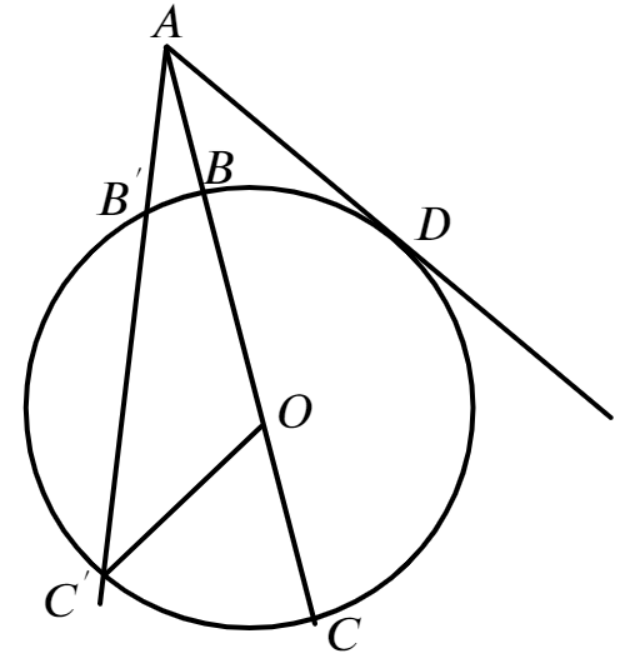
\includegraphics[scale=0.35]{g9-31.png}}
\end{figure}\\
Сначала покажем, что наибольшая секущая проходит через центр окружности. Проведём проходящую через центр секущую $AC$ и какую-то другую секущую $AC'.$ Тогда по неравенству треугольника для треугольника $AOC'$ имеем $AC'<AO+OC'=AO+OC=AC,$ ч.т.д. Пусть радиус окружности равен $R,$ а $AB=x.$ По свойству касательной и секущей
запишем равенство $AD^2=AB\cdot AC,\ 400=x\cdot 50,\ x=8$см, при этом $x+2R=50,\ R=21$см.\\
